\lab{Algorithms}{IVP Solvers}{IVP Solvers}
\label{lab:IVP}

\objective{Implement several basic numerical solvers for initial value problems.}

Consider the initial value problem 
\begin{eqnarray*}
y' &=& f(x,y), a \leq x \leq b, \\
y(a) &=& y_0.
\end{eqnarray*}
A solution is a differentiable function $y(x)$ that satisfies the equation $y' = f(x,y)$ on the interval $[a,b]$ and for which $y(a) = y_0$.  There are many initial value problems (IVPs) where it is impossible to find a closed form expression for the solution. In these cases especially it is important to be able to use various methods of numerical approximation to study a solution which we know does exist. 

Most methods require us to approximate the solution on a set of grid points $a = x_0< x_1<\hdots< x_n = b$ in our interval.  For simplicity we will assume that each of the $n$ subintervals $[x_{i-1},x_i]$ has equal length $h = (b-a)/n$. $h$ is called the \textit{step size}. We then look for values $y_0,y_1, \hdots, y_n$ that approximate our solution ( so $y_i \approx y(x_i)$).  

Perhaps the simplest way to find the values $y_i$ is to use Taylor's theorem. For each $i, 1 \leq i \leq n$, 
\begin{eqnarray*}
y(x_{i+1}) &=& y(x_{i}) + h y'(x_i) + \frac{h^2}{2} y''(\xi_i), \xi_i \in [x_i,x_{i+1}], \\
y(x_{i+1}) &=& y(x_{i}) + h f(x_i,y(x_i)) + \frac{h^2}{2} y''(\xi_i),\\
y(x_{i+1}) &\approx & y(x_{i}) + h f(x_i,y(x_i)) \text{ for small } h .
\end{eqnarray*}
This approximation leads to a first order method called Euler's method: 
\begin{enumerate}
\item Let $y_0 = y(a)$. 
\item For $i = 0, 1, \hdots, n-1$, let $y_{i+1} = y_i +hf(x_i,y_i)$. 
\end{enumerate}

We can also use Taylor's theorem as follows: 
\begin{eqnarray*}
y(x_{i}) &=& y(x_{i+1}) - h y'(x_{i+1}) + \frac{h^2}{2} y''(\xi_i), \xi_i \in [x_i,x_{i+1}], \\
y(x_{i}) &=& y(x_{i+1}) + h f(x_{i+1},y(x_{i+1})) + \frac{h^2}{2} y''(\xi_i),\\
y(x_{i+1}) &\approx & y(x_{i}) + h f(x_{i+1},y(x_{i+1}))  \text{ for small } h .
\end{eqnarray*}
This approximation leads to backwards Euler's method, another first order method: 
\begin{enumerate}
\item Let $y_0 = y(a)$. 
\item For $i = 0, 1, \hdots, n-1$, solve  $y_{i} = y_{i+1}-hf(x_{i+1},y_{i+1})$ for $y_{i+1}$. 
\end{enumerate}

Note that for both the Euler and backwards Euler methods, only $x_i, y_i,$ and $f(x_i,y_i)$ are needed to find $y_{i+1}$. Because of this these are called \textit{one-step methods}. 



%\clearpage

\begin{figure}[ht]
\centering
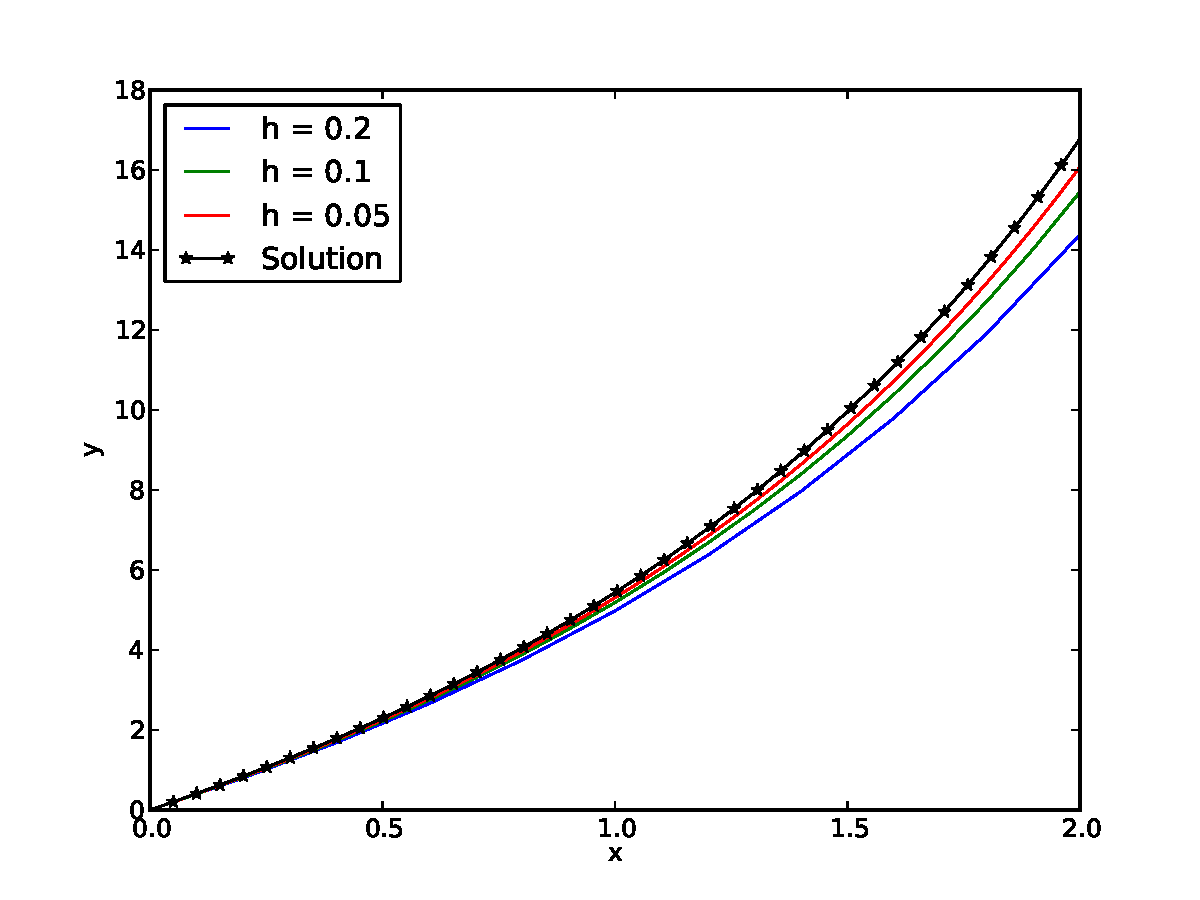
\includegraphics[width=\textwidth]{Fig1.pdf}
\caption{The solution of $y' -y= -2x+4, y(0) = 0$, is $y(x) = -2+2x + 2e^x.$ This is a plot of the solution, alongside approximations with Euler's method for several stepsizes.}
\label{ivp:euler}
\end{figure}



\begin{problem}
The solution of the IVP
\begin{eqnarray*}
y' + y &=& 2-2x,\,\, 0 \leq x \leq 2, \\
y(0) &=& 0,
\end{eqnarray*}
is given by $y(x) = 4-2x -4e^{-x}$. Use Euler's method to numerically approximate the solution
with step sizes $h = 0.4, 0.2$, and $0.1.$ Plot your results using \li{matplotlib}.
\end{problem}



So how do we come up with numerical methods with higher order accuracy? Using Taylor's theorem (as we did for Euler's method) to create higher-order one-step methods would lead to numerically approximating derivatives of $f(t,y)$ - not necessarily desirable. 

Let us look for a second order method of the form 
\begin{enumerate}
\item $y_0 = y(a)$,
\item $y_{i+1} = y_i + a f(x_i+b, y_i+c)$.
\end{enumerate}
By expanding $a f(x+b, y+c)$ with Taylor's theorem and matching constants with 
\begin{eqnarray*}
f(x,y) + \frac{h}{2}f'(x,y) &=& f(x,y) + \frac{h}{2}\frac{\partial f}{\partial x}(x,y) +  + \frac{h}{2}\frac{\partial f}{\partial y}(x,y) \cdot f(x,y),
\end{eqnarray*}
we find that $a = 1, b = h/2,$ and $c = h/2$. This method is called the Midpoint method. IVP solvers with this general form are called \textit{Runge-Kutta methods}. Another second order (Runge-Kutta) method is the modified Euler method: 
\begin{enumerate}
\item $y_0 = y(a)$,
\item $y_{i+1} = y_i + \frac{h}{2}[ f(x_i, y_i) + f(x_{i+1}, y_i+ hf(x_i, y_i))]$ for $i = 0,1,\hdots, n-1$. 
\end{enumerate}

There are many Runge-Kutta methods with varying orders of accuracy. In practice, the methods of order four, such as the following, are most commonly used: 
\begin{enumerate}
\item $y_0 = y(a)$, 
\item $K_1 = hf(x_i,y_i)$,
\item $K_2 = hf(x_i + \frac{h}{2}, y_i + \frac{1}{2} K_1),$
\item $K_3 = hf(x_i + \frac{h}{2} , y_i + \frac{1}{2} K_2),$
\item $K_4 = hf(x_{i+1} , y_i +  K_3),$
\item $y_{i+1} = y_i + \frac{1}{6}(K_1 + K_2 + K_3 + K_4)$ for $i = 0,1,\hdots,n-1$.
\end{enumerate}




\begin{problem}
Suppose a differential equation is given by
\[ y' = f(t).\]
Which quadrature formulas correspond to Euler's method, backward Euler's method, modified Euler's method, the Midpoint method, and the fourth order Runge-Kutta method (RK4)? 
\end{problem}


\begin{problem}
Consider the IVP given by 
\begin{eqnarray*}
y' + y &=& 2-2x,\,\, 0 \leq x \leq 2, \\
y(0) &=& 0.
\end{eqnarray*}
Use Euler's method, the Midpoint method, and RK4 to approximate the value of the solution at $x = 2$, with a stepsize of $h = 0.2, 0.1,$ and $0.05 $. Find the relative error of each approximation.
\end{problem}

For many differential equations $y' = f(x,y)$ there is no closed form expression. Even when there is a closed form expression, it may be difficult to interpret. Consider the initial value problem 
\begin{eqnarray*}
y'(x) &=& \sin y(x), \\
y(0) &=& y_0.
\end{eqnarray*}
This IVP has an implicit solution given by 
\[x = \ln \left|\frac{\cos y_0 + \cot y_0}{\csc y + \cot y} \right|.\]
In this case, and many others, to understand the general solution of a ordinary differential equation it is often easier to use an IVP solver to plot several integral curves for various initial values. For example, it is easy to show that this differential equation has constant solutions $y_n(x) = n \pi, n \in \mathbb{N}$. Knowing this, and plotting several integral curves as in the following figure, it is easy to see how solutions of this IVP will behave.


\begin{figure}
\centering
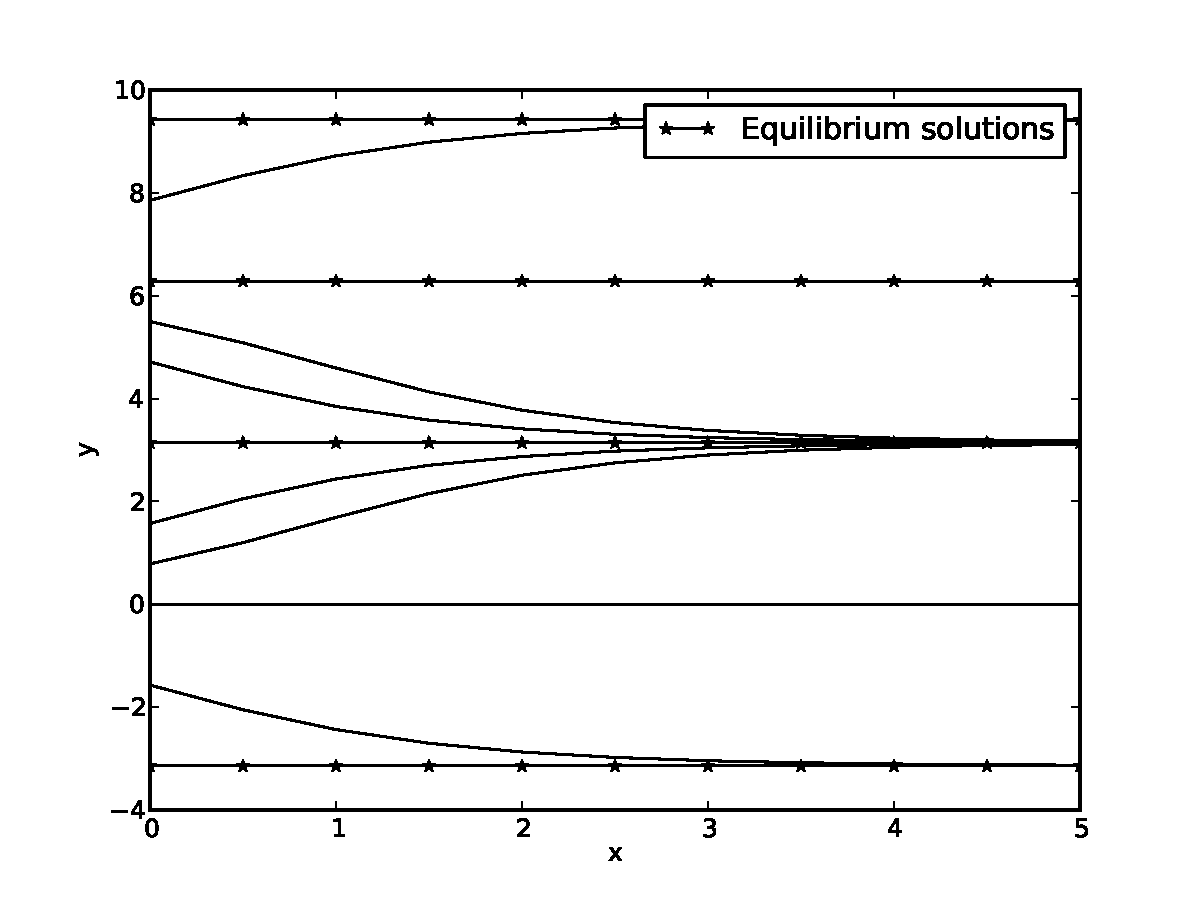
\includegraphics[width=\textwidth]{Fig4.pdf}
\caption{Several integral curves for the differential equation $y' =\sin y$, using the python solver \li{dopri5}. }
\label{ivp:int_curves}
\end{figure}

\begin{problem}
Plot the solutions of 
\[ y' + y = 2-2x\,\, 0 \leq x \leq 2, \] 
with initial conditions $y(0) = 0, 2, 4, 6, $ and $8$. Use RK4 to compute the solutions. 
\end{problem}



%References:
%
%Perona, Pietro, and Jitendra Malik. "Scale-Space and Edge Detection Using Anisotropic Diffusion." IEE Transactions on Pattern Analysis and Machine Intelligence 12 (1990): 629-39. Web.
%
%Kim, Seongjai. "Edge-Preserving Noise Removal, Part I: Second Order Anisotropic Diffusion." University of Kentucky Department of Mathematics Technical Report (2009): n. pag. Web.
%
